\hypertarget{realCompare_8c}{
\section{real\-Compare.c File Reference}
\label{realCompare_8c}\index{realCompare.c@{realCompare.c}}
}
{\tt \#include \char`\"{}real\-Compare.h\char`\"{}}\par


Include dependency graph for real\-Compare.c:\begin{figure}[H]
\begin{center}
\leavevmode
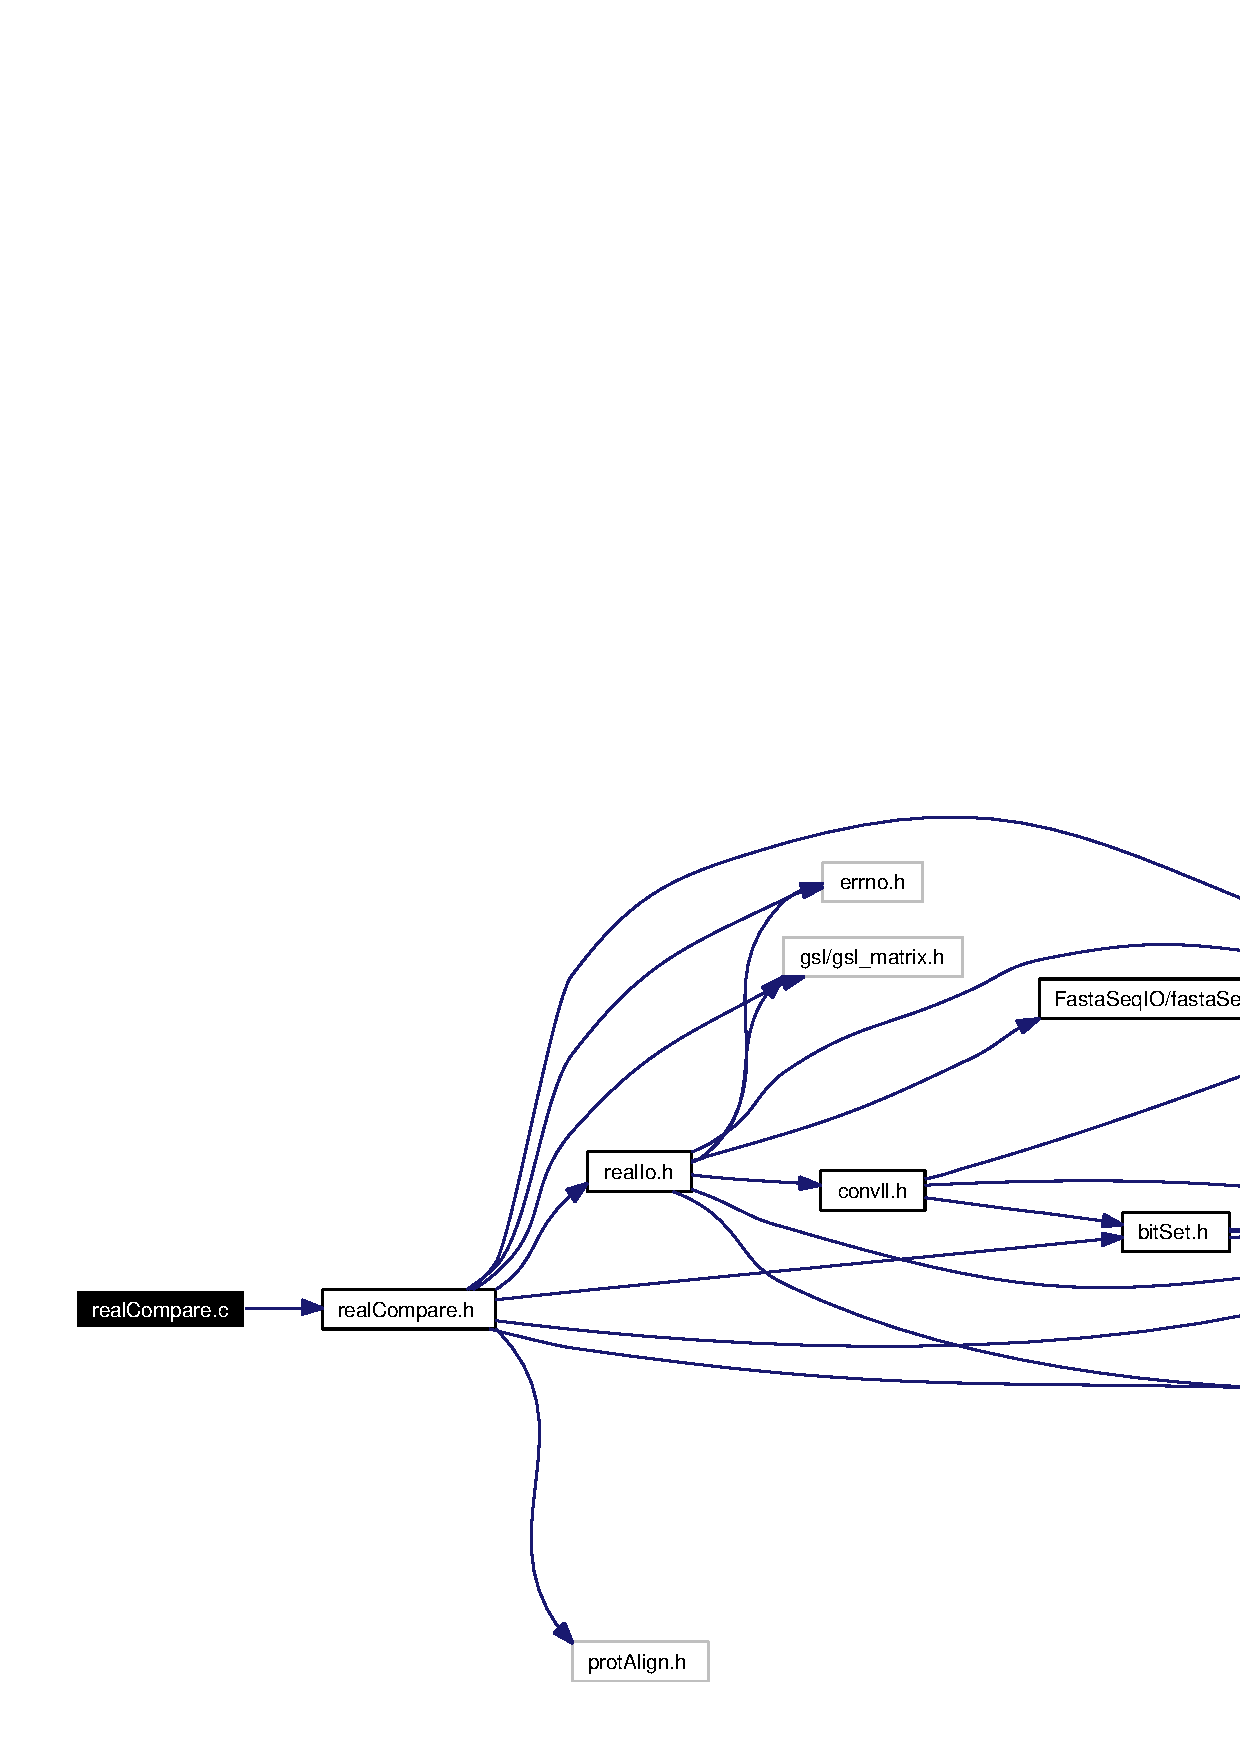
\includegraphics[width=358pt]{realCompare_8c__incl}
\end{center}
\end{figure}
\subsection*{Functions}
\begin{CompactItemize}
\item 
double \hyperlink{realCompare_8c_a0}{rmsd\-Compare} (\hyperlink{structrdh__t}{rdh\_\-t} $\ast$data, int win1, int win2, int L, double $\ast$extra\-Params)
\item 
double \hyperlink{realCompare_8c_a1}{general\-Match\-Factor} (\hyperlink{structrdh__t}{rdh\_\-t} $\ast$data, int win1, int win2, int L, double $\ast$extra\-Params)
\item 
double \hyperlink{realCompare_8c_a2}{mass\-Spec\-Compare\-WElut} (\hyperlink{structrdh__t}{rdh\_\-t} $\ast$data, int win1, int win2, int L, double $\ast$extra\-Params)
\item 
double($\ast$)(\hyperlink{structrdh__t}{rdh\_\-t} $\ast$, int, int, int, double $\ast$) \hyperlink{realCompare_8c_a3}{get\-Comp\-Func} (int comp\-Func)
\item 
\hyperlink{structbitGraph__t}{bit\-Graph\_\-t} $\ast$ \hyperlink{realCompare_8c_a4}{real\-Comparison} (\hyperlink{structrdh__t}{rdh\_\-t} $\ast$data, int L, double g, int comp\-Func, double $\ast$extra\-Params)
\end{CompactItemize}


\subsection*{Detailed Description}
This file defines a series of functions that are used during the comparison phase of the Gemoda algorithm in the real valued implementation. We define a handful of comparison functions --- some that are well suited to protein structure comparison and others that are more suited to the comparison of mass spectrometry spectra.

Definition in file \hyperlink{realCompare_8c-source}{real\-Compare.c}.

\subsection*{Function Documentation}
\hypertarget{realCompare_8c_a1}{
\index{realCompare.c@{real\-Compare.c}!generalMatchFactor@{generalMatchFactor}}
\index{generalMatchFactor@{generalMatchFactor}!realCompare.c@{real\-Compare.c}}
\subsubsection[generalMatchFactor]{\setlength{\rightskip}{0pt plus 5cm}double general\-Match\-Factor (\hyperlink{structrdh__t}{rdh\_\-t} $\ast$ {\em data}, int {\em win1}, int {\em win2}, int {\em L}, double $\ast$ {\em extra\-Params})}}
\label{realCompare_8c_a1}


This function is used to compute a generalized match factor, which is useful for computing the degree of similarity between mass spectrometry spectra.

Definition at line 111 of file real\-Compare.c.

References get\-Rdh\-Dim(), get\-Rdh\-Index\-Seq\-Pos(), and rdh\_\-t::seq.

Referenced by get\-Comp\-Func().

\scriptsize\begin{verbatim}113 {
114   int i, j;
115   double numerator = 0.0;
116   
117     /*
118        double denominator=0.0;
119      */ 
120   double xsum;
121   double ysum;
122   double ldenom = 0.0;
123   double rdenom = 0.0;
124   int dim;
125   int seq1, pos1;
126   int seq2, pos2;
127   gsl_matrix_view view1;
128   gsl_matrix_view view2;
129   gsl_matrix * mat1;
130   gsl_matrix * mat2;
131   dim = getRdhDim (data);
132   
133     // Find out which seq,pos pairs these two
134     // windows correspond to
135     getRdhIndexSeqPos (data, win1, &seq1, &pos1);
136   getRdhIndexSeqPos (data, win2, &seq2, &pos2);
137   
138     // Get a reference to a submatrix.  That is,
139     // 'chop out' the window.
140     view1 = gsl_matrix_submatrix (data->seq[seq1], pos1, 0, L, dim);
141   view2 = gsl_matrix_submatrix (data->seq[seq2], pos2, 0, L, dim);
142   
143     // Some error checking here would be nice!
144     // Did we get the matrices we wanted?
145     
146     // This just makes it easier to handle the views
147     mat1 = &view1.matrix;
148   mat2 = &view2.matrix;
149   
150     // Loop over each position
151     for (i = 0; i < mat1->size1; i++)
152     {
153       xsum = 0.0;
154       ysum = 0.0;
155       
156     // Loop over each dimension at each position
157     for (j = 0; j < dim; j++)
158     {
159       xsum += gsl_matrix_get (mat1, i, j);
160       ysum += gsl_matrix_get (mat2, i, j);
161     }
162       numerator += (i + 1) * sqrt (xsum * ysum);
163       ldenom += (i + 1) * xsum;
164       rdenom += (i + 1) * ysum;
165     }
166   return pow (numerator, 2.0) / (ldenom * rdenom);
167 }
\end{verbatim}
\normalsize 


\hypertarget{realCompare_8c_a3}{
\index{realCompare.c@{real\-Compare.c}!getCompFunc@{getCompFunc}}
\index{getCompFunc@{getCompFunc}!realCompare.c@{real\-Compare.c}}
\subsubsection[getCompFunc]{\setlength{\rightskip}{0pt plus 5cm}double($\ast$)(\hyperlink{structrdh__t}{rdh\_\-t} $\ast$, int, int, int, double $\ast$) get\-Comp\-Func ()}}
\label{realCompare_8c_a3}




Definition at line 264 of file real\-Compare.c.

References general\-Match\-Factor(), mass\-Spec\-Compare\-WElut(), and rmsd\-Compare().

\scriptsize\begin{verbatim}265 {
266   double (*comparisonFunc) (rdh_t *, int, int, int, double *) = &rmsdCompare;
267   switch (compFunc)
268     {
269     case 0:
270       comparisonFunc = &rmsdCompare;
271       break;
272     case 1:
273       comparisonFunc = &generalMatchFactor;
274       break;
275     case 2:
276       comparisonFunc = &massSpecCompareWElut;
277       break;
278     default:
279       comparisonFunc = &rmsdCompare;
280       break;
281     }
282   return (comparisonFunc);
283 }
\end{verbatim}
\normalsize 


\hypertarget{realCompare_8c_a2}{
\index{realCompare.c@{real\-Compare.c}!massSpecCompareWElut@{massSpecCompareWElut}}
\index{massSpecCompareWElut@{massSpecCompareWElut}!realCompare.c@{real\-Compare.c}}
\subsubsection[massSpecCompareWElut]{\setlength{\rightskip}{0pt plus 5cm}double mass\-Spec\-Compare\-WElut (\hyperlink{structrdh__t}{rdh\_\-t} $\ast$ {\em data}, int {\em win1}, int {\em win2}, int {\em L}, double $\ast$ {\em extra\-Params})}}
\label{realCompare_8c_a2}


This function is used to compute the match factor between to mass spectrometry spectra in a similar manner to the previous function; however, this function imposes a penalty for spectra that are separated by large distances in elution time. This function is commonly used by Spec\-Connect.

Definition at line 178 of file real\-Compare.c.

References get\-Rdh\-Dim(), get\-Rdh\-Index\-Seq\-Pos(), and rdh\_\-t::seq.

Referenced by get\-Comp\-Func().

\scriptsize\begin{verbatim}180 {
181   int i, j;
182   double numerator = 0.0;
183   
184     /*
185        double denominator=0.0;
186      */ 
187   double xsum;
188   double ysum;
189   double cum;
190   double ldenom = 0.0;
191   double rdenom = 0.0;
192   int dim;
193   int seq1, pos1;
194   int seq2, pos2;
195   double weight = 2.0;
196   gsl_matrix_view view1;
197   gsl_matrix_view view2;
198   gsl_matrix * mat1;
199   gsl_matrix * mat2;
200   double maxElut = -1;
201   if (extraParams != NULL)
202     {
203       maxElut = extraParams[0];
204     }
205   dim = getRdhDim (data);
206   
207     // Find out which seq,pos pairs these two
208     // windows correspond to
209     getRdhIndexSeqPos (data, win1, &seq1, &pos1);
210   getRdhIndexSeqPos (data, win2, &seq2, &pos2);
211   
212     // Get a reference to a submatrix.  That is,
213     // 'chop out' the window.
214     view1 = gsl_matrix_submatrix (data->seq[seq1], pos1, 0, L, dim);
215   view2 = gsl_matrix_submatrix (data->seq[seq2], pos2, 0, L, dim);
216   
217     // Some error checking here would be nice!
218     // Did we get the matrices we wanted?
219     
220     // This just makes it easier to handle the views
221     mat1 = &view1.matrix;
222   mat2 = &view2.matrix;
223   cum = 1.0;
224   
225     // Loop over each position
226     for (i = 0; i < mat1->size1; i++)
227     {
228       xsum = 0.0;
229       ysum = 0.0;
230       
231     // First take the first dimension for elution time
232     if (maxElut >= 0)
233     {
234       if (fabs
235            (gsl_matrix_get (mat1, i, 0) - gsl_matrix_get (mat2, i, 0)) >
236            maxElut)
237         {
238           cum = 0;
239           break;
240         }
241     }
242       
243     // printf("\n");
244     // 
245     // Loop over each subsequent dimension at each position
246     for (j = 1; j < dim; j++)
247     {
248       
249         // printf("mat1val=%lf,mat2val=%lf\n",gsl_matrix_get(mat1,i,j),
250         // gsl_matrix_get(mat2,i,j));
251         numerator += pow (j, weight) * sqrt (gsl_matrix_get (mat1, i, j) 
252                          *gsl_matrix_get (mat2, i,
253                                   j));
254       ldenom += pow (j, weight) * gsl_matrix_get (mat1, i, j);
255       rdenom += pow (j, weight) * gsl_matrix_get (mat2, i, j);
256       
257         // printf("numer=%lf,ldenom=%lf,rdenom=%lf\n",numerator,
258         // ldenom,rdenom);
259     }
260       cum *= pow (numerator, 2.0) / (ldenom * rdenom);
261     }
262   return pow (cum, 1.0 / L);
263 }
\end{verbatim}
\normalsize 


\hypertarget{realCompare_8c_a4}{
\index{realCompare.c@{real\-Compare.c}!realComparison@{realComparison}}
\index{realComparison@{realComparison}!realCompare.c@{real\-Compare.c}}
\subsubsection[realComparison]{\setlength{\rightskip}{0pt plus 5cm}\hyperlink{structbitGraph__t}{bit\-Graph\_\-t}$\ast$ real\-Comparison (\hyperlink{structrdh__t}{rdh\_\-t} $\ast$ {\em data}, int {\em L}, double {\em g}, int {\em comp\-Func}, double $\ast$ {\em extra\-Params})}}
\label{realCompare_8c_a4}




Definition at line 285 of file real\-Compare.c.

References bit\-Graph\-Set\-True\-Sym(), get\-Comp\-Func, get\-Rdh\-Index\-Seq\-Pos(), rdh\_\-t::index\-Size, init\-Rdh\-Index(), new\-Bit\-Graph(), and rmsd\-Compare().

Referenced by main().

\scriptsize\begin{verbatim}287 {
288   int i, j;
289   int seq1, pos1;
290   int seq2, pos2;
291   bitGraph_t * bg = NULL;
292   double score;
293   double (*comparisonFunc) (rdh_t *, int, int, int, double *) = &rmsdCompare;
294   
295     // Initialize the rdh's index
296     initRdhIndex (data, L, 1);
297   
298     // Allocate a new bit graph
299     bg = newBitGraph (data->indexSize);
300   
301     // Choose the comparison function, pass a reference to it
302     comparisonFunc = getCompFunc (compFunc);
303   for (i = 0; i < data->indexSize; i++)
304     {
305       
306     // Skip seperators
307     getRdhIndexSeqPos (data, i, &seq1, &pos1);
308       if (seq1 == -1 || pos1 == -1)
309     {
310       continue;
311     }
312       for (j = i; j < data->indexSize; j++)
313     {
314       getRdhIndexSeqPos (data, j, &seq2, &pos2);
315       if (seq2 == -1 || pos2 == -1)
316         {
317           continue;
318         }
319       
320         // This is the comparison function
321         score = comparisonFunc (data, i, j, L, extraParams);
322       
323         // printf("score (%2d,%2d) vs. (%2d, %2d) =\t%lf\n",seq1, pos1, seq2, pos2,
324         // score);
325         if (compFunc == 0)
326         {
327           if (score <= g)
328         {
329           bitGraphSetTrueSym (bg, i, j);
330         }
331         }
332       else if ((compFunc == 1) || (compFunc == 2))
333         {
334           if (score >= g)
335         {
336           bitGraphSetTrueSym (bg, i, j);
337         }
338         }
339       else
340         {
341           fprintf (stderr, "Comparison function undefined in " 
342             "realComparison function,\n located in " 
343             "realCompare.c.  Exiting.\n\n");
344           fflush (stderr);
345           exit (0);
346         }
347     }
348     }
349   return bg;
350 }
\end{verbatim}
\normalsize 


\hypertarget{realCompare_8c_a0}{
\index{realCompare.c@{real\-Compare.c}!rmsdCompare@{rmsdCompare}}
\index{rmsdCompare@{rmsdCompare}!realCompare.c@{real\-Compare.c}}
\subsubsection[rmsdCompare]{\setlength{\rightskip}{0pt plus 5cm}double rmsd\-Compare (\hyperlink{structrdh__t}{rdh\_\-t} $\ast$ {\em data}, int {\em win1}, int {\em win2}, int {\em L}, double $\ast$ {\em extra\-Params})}}
\label{realCompare_8c_a0}


Calculate the rmsd between two windows, with optional translation and rotation. The input to this function is a real data handler object, two integers that point to the windows within the real data that are to be compared, an integer that specifies the length of the windows, and a pointer to a double precision floating point that can be used to store other parameters as needed. This last parameter is most useful for implementing other comparison functions, without having to make, too many changes to other parts of the code.

This function operates in three stages. First, we compute the centroid of each window and move the second window such that its centroid overlaps with that of the first window. Second, we use rigid body rotation to find the rotational matrix that minimizes the root mean squared deviation between the two windows. Finally, this function returns that minimized RMSD.

Definition at line 31 of file real\-Compare.c.

References get\-Rdh\-Dim(), get\-Rdh\-Index\-Seq\-Pos(), and rdh\_\-t::seq.

Referenced by get\-Comp\-Func(), and real\-Comparison().

\scriptsize\begin{verbatim}32 {
33   int trans = 1;
34   int rot = 1;
35   int dim;
36   double result = 0;
37   int seq1, pos1;
38   int seq2, pos2;
39   gsl_matrix_view view1;
40   gsl_matrix_view view2;
41   gsl_matrix * mat1;
42   gsl_matrix * mat2;
43   gsl_matrix * mat1copy;
44   gsl_matrix * mat2copy;
45   
46     // The "rint" function is in math.h and rounds a number to the 
47     // nearest integer.  It raises an "inexact exception" if the
48     // number initially wasn't an integer.
49     if (extraParams != NULL)
50     {
51       trans = rint (extraParams[0]);
52       rot = rint (extraParams[1]);
53     }
54   dim = getRdhDim (data);
55   
56     // Find out which seq,pos pairs these two
57     // windows correspond to
58     getRdhIndexSeqPos (data, win1, &seq1, &pos1);
59   getRdhIndexSeqPos (data, win2, &seq2, &pos2);
60   
61     // Get a reference to a submatrix.  That is,
62     // 'chop out' the window.
63     view1 = gsl_matrix_submatrix (data->seq[seq1], pos1, 0, L, dim);
64   view2 = gsl_matrix_submatrix (data->seq[seq2], pos2, 0, L, dim);
65   
66     // This just makes it easier to handle the views
67     mat1 = &view1.matrix;
68   mat2 = &view2.matrix;
69   
70     // Create copies of the windows, because our comparison
71     // will require altering the matrices
72     mat1copy = gsl_matrix_alloc (mat1->size1, mat1->size2);
73   mat2copy = gsl_matrix_alloc (mat2->size1, mat2->size2);
74   gsl_matrix_memcpy (mat1copy, mat1);
75   gsl_matrix_memcpy (mat2copy, mat2);
76   
77     /*
78         printf("matrix1:\n"); gsl_matrix_pretty_fprintf(stdout, mat1copy, "%f ");
79        printf("\nmatrix2:\n"); gsl_matrix_pretty_fprintf(stdout, mat2copy, "%f "); 
80      */ 
81     
82     // Are we going to do a translation?
83     if (trans == 1)
84     {
85       moveToCentroid (mat1copy);
86       moveToCentroid (mat2copy);
87     }
88   
89     // Are we going to do a rotation?
90     if (rot == 1)
91     {
92       
93     // Rotate mat2copy to have a minimal
94     // rmsd with mat1copy
95     rotateMats (mat1copy, mat2copy);
96     }
97   
98     // Compute the rmsd between mat2copy and mat2copy
99     result = gsl_matrix_rmsd (mat1copy, mat2copy);
100   gsl_matrix_free (mat1copy);
101   gsl_matrix_free (mat2copy);
102   return result;
103 }
\end{verbatim}
\normalsize 


